Sezione di \emph{Strumenti per sviluppatori} del browser Google Chrome.\\
Permette di identificare e risolvere i problemi inerenti alle performance del sito, all'accessibilità, all'esperienza utente e la SEO (Search Engine Optimization).\\
E' possibile verificare il sito da dispositivo mobile o desktop, e selezionare le varie verifiche. Nel nostro caso, la verifica \emph{Progressive Web App} non ci interessa in quanto il nostro progetto non è un applicazione Web che si carica come una normale pagina Web, ma un semplice sito Web.\\
Cliccando \emph{Run audits}, si accede al pannello dove vengono visualizzati i risultati in percentuale e le possibili correzioni da attuare.
\begin{figure}[!h]
	\centering
	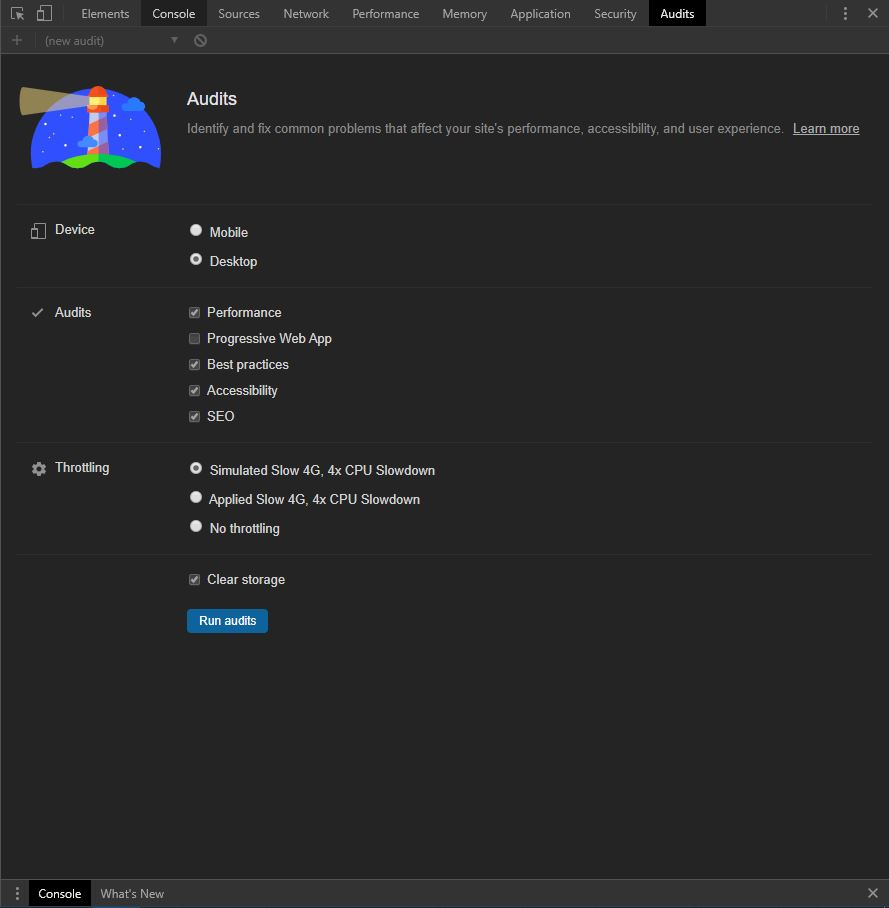
\includegraphics[width=0.7\linewidth]{sezioni/FaseTest/Immagini/audits.JPG}\\
	\caption{Strumenti per sviluppatori Google Chrome: Audits}
	\label{Fig:audits}
\end{figure}

\newpage